\section{Introduction}

Provide a general introduction to the area for the degree project. Use references!

Link things together with references. This is a reference to a section: \ref{sec:background}.

\subsection{Background}
\label{sec:background}
Present the background for the area. Give the context by explaining the parts that are needed to understand the degree project and thesis. (Still, keep in mind that this is an introductory part, which does not require too detailed description).

Use references\footnote{You can also add footnotes if you want to clarify the content on the same page.}

Detailed description of the area should be moved to Chapter 2, where detailed information about background is given together with related work. 

This background presents background to writing a report in latex.


Example citation \cite{Jones2017} or for two authors: \cite{Jones2017, Liu2017}

Look at sample table \ref{tab:sample-table-label} for a table sample.

\begin{table}[!ht]
\centering
\caption{Sample table. Make sure the column with adds up to 0.94 for a nice look.}
~\\
\label{tab:sample-table-label}
\begin{tabular}{p{0.3\textwidth} p{0.64\textwidth}}
\toprule
\textbf{SAMPLE}		  & \textbf{TABLE}                                                                                                                                                  \\ \toprule
One                   & Stuff 1 \\
\midrule
Two                   & Stuff 2 \\
\midrule
Three                 & Stuff 3\\
\bottomrule
\end{tabular}
\end{table}



Boxes can be used to organize content

\begin{tcolorbox}[title={Development environment for prototype}]
	\tt{
		\textbf{Operating systems }\\
		computer: Linux - kernel 4.18.5-arch1-1-ARCH\\
		android phone: 8.1.0\\
		~\\
		\textbf{Build tools}\\
		exp (build tool): version 55.0.4\\
		~\\
		...
	}
\end{tcolorbox}


Multiple images can be placed side by side like this:
\begin{figure}[ht]
	\centering 
	\subfloat[First subfigure]{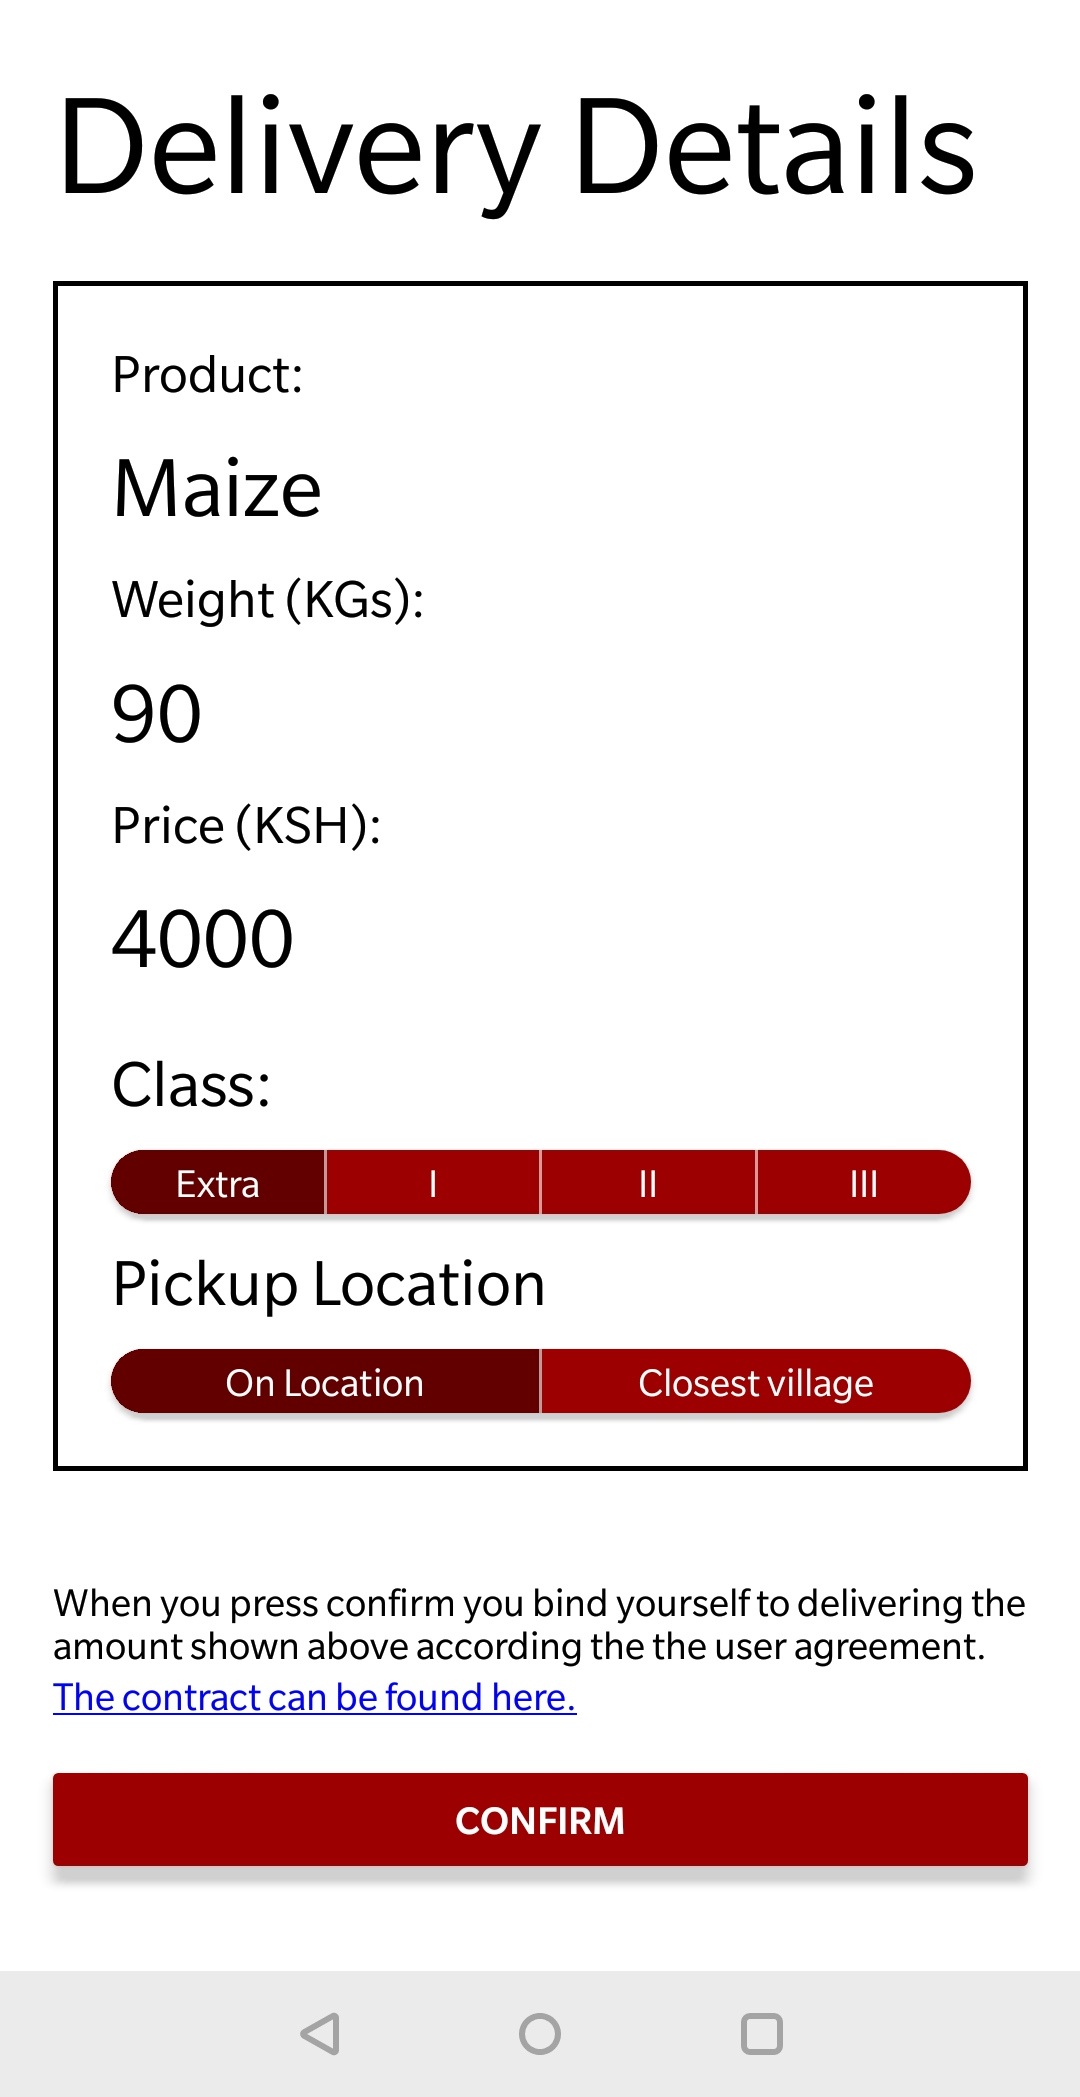
\includegraphics[width=0.3\textwidth]{img/sample-image}
		\label{fig:sample-image:1}}
	\hfill
	\subfloat[Second subfigure]{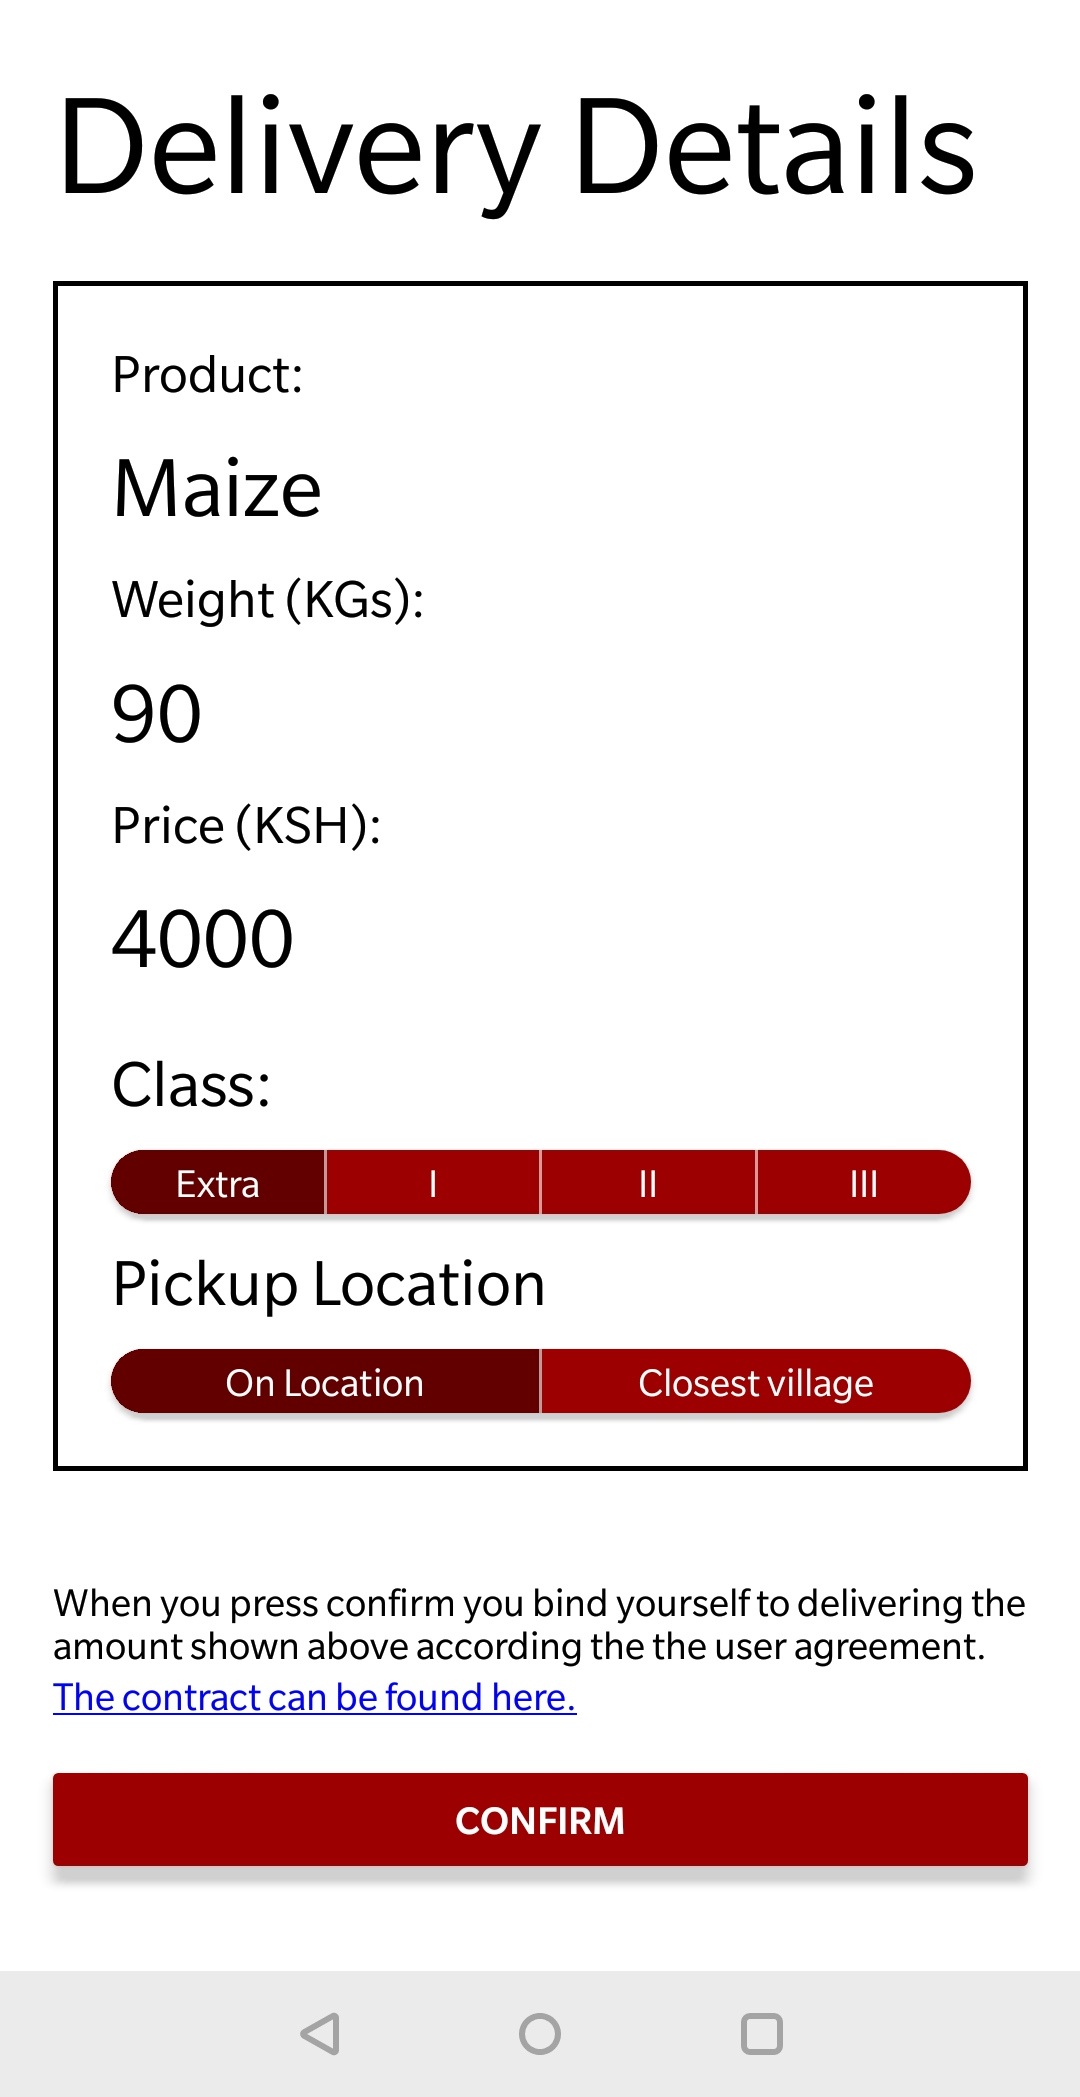
\includegraphics[width=0.3\textwidth]{img/sample-image}
		\label{fig:sample-image:2}}
	\hfill
	\subfloat[Third subfigure]{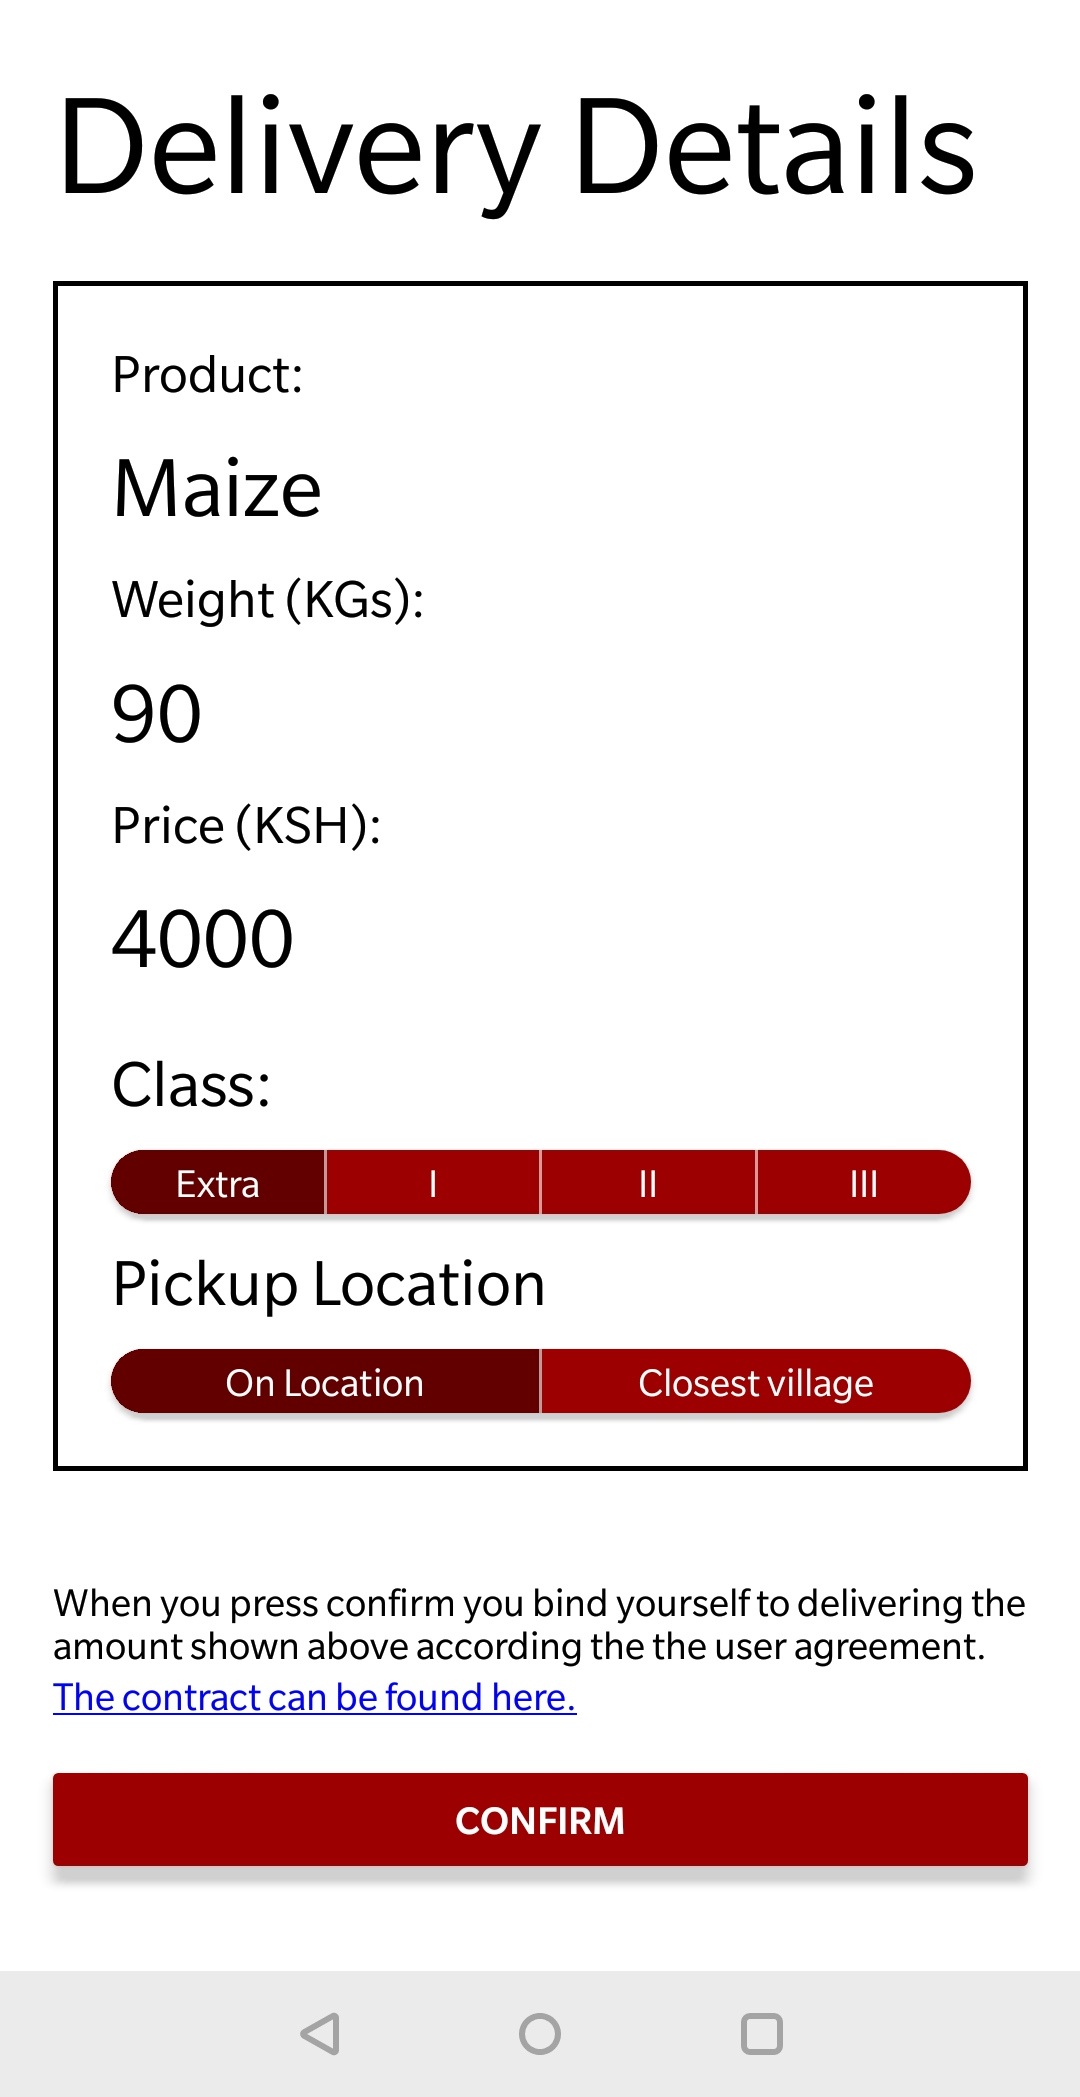
\includegraphics[width=0.3\textwidth]{img/sample-image}
		\label{fig:sample-image:3}}
	\caption{\textit{General figure caption. The width might not add up to 1. Try make sure it adds up to 0.9 instead.}}
\end{figure}

\subsection{Problem}
Present the problems found in the area. Preferable use and end this section with a question as a problem statement.

Use references
Preferable, state the problem, to be solved, as a question. Do not use a question that can be answered with yes and/or no. 

\subsection{Purpose}
The purpose of the degree project/thesis is the purpose of the written material, i.e., the thesis. The thesis presents the work / discusses / illustrates and so on.

It is not “The project is about” even though this can be included in the purpose. If so, state the purpose of the project after purpose of the thesis).

\subsection{Goal}
The goal means the goal of the degree project. Present following: the goal(s), deliverables and results of the project. 

\subsubsection{Benefits, Ethics and Sustainability}
Describe who will benefit from the degree project, the ethical issues (what ethical problems can arise) and the sustainability aspects of the project.

Use references!

\subsection{Methodology}
Introduce, theoretically, the methodologies and methods that can be used in a project and, then, select and introduce the methodologies and methods that are used in the degree project. Must be described on the level that is enough to understand the contents of the thesis. 

Use references!

Preferably, the philosophical assumptions, research methods, and research approaches are presented here. Write quantitative / qualitative, deductive / inductive / abductive. Start with theory about methods, choose the methods that are used in the thesis and apply. 


Detailed description of these methodologies and methods should be presented in Chapter 3. In chapter 3, the focus could be research strategies, data collection, data analysis, and quality assurance.


\subsection{Stakeholders}
Present the stakeholders for the degree project.

\subsection{Delimitations}
Explain the delimitations. These are all the things that could affect the study if they were examined and included in the degree project. 
Use references!

\subsection{Outline}
In text, describe what is presented in Chapters 2 and forward. Exclude the first chapter and references as well as appendix. 
